%!TEX root = volumeFinal.tex 
\chapter{\label{chap:planejamento}Planejamento}

\frm[inline]{Sempre que citar livro, dizer capítulo e páginas}
Planejamento automatizado é uma área da inteligencia artificial que estuda o processo de geração de planos de forma computacional. Este tipo de planejamento está preocupado com a forma geral da composição dos planos \cite{ghallab2004automated}. O planejamento na computação se diferencia das outras áreas pelo fato de que todo o plano é gerado automaticamente. 

Uma entrada necessária para qualquer algoritmo de planejamento é a representação do problema a ser resolvido. A representação de um problema é onde estão descritos os estados e as transições dos estados. Um estado do sistema é representados por um conjunto de átomos que resultam em verdadeiro ou falso dependendo da interpretação do ambiente. Para determinar as transições dos estados são utilizadas ações que são  representadas por operadores de planejamento que alteram os valores dos átomos presentes em determinado estado. Um operador de planejamento é definido como \textit{op} = (nome(\textit{op}), precondições(\textit{op}), efeitos(\textit{op})), onde cada elemento é definido como \cite{ghallab2004automated}: 

\begin{itemize}
	\item nome(\textit{op}) - É o nome do operador de planejamento e \textit{op} é o conjunto de todas as variáveis que irão aparecer qualquer parte do operador de planejamento.  
	\item precondições(\textit{op}) - \textit{op} é o conjunto de átomos ou átomos negativos que representa a precondição do operador de planejamento. 
	\item efeitos(\textit{op}) - \textit{op} é o conjunto de átomos ou átomos negativos que representa o efeito do operador de planejamento
\end{itemize}

O nome deve ser único pelo proposito de o nome poder se referir ao operador por completo, ou seja, após definido apenas com o nome pode-se inferir as pré e pós condições, assim escrevendo o nome(\textit{op}) para se referir a todo o operador de planejamento \textit{op}. 

Um problema de planejamento é descrito como \textit{P} = \textit{($\Sigma$, $s_{0}$, g)}. Onde $\Sigma$ é a representação do problema, $s_{0}$ é o estado inicial, estado onde o problema começa, e g é o objetivo, estado onde o problema deve acabar. Um planejador é responsável por pegar essas informações e gerar um plano que comece pelo estado inicial e chegue ao objetivo através de um conjunto de ações descritas na representação do problema. A figura \ref{fig:planmodelo} representa esse processo.

\begin{figure}[ht]
	\centering
	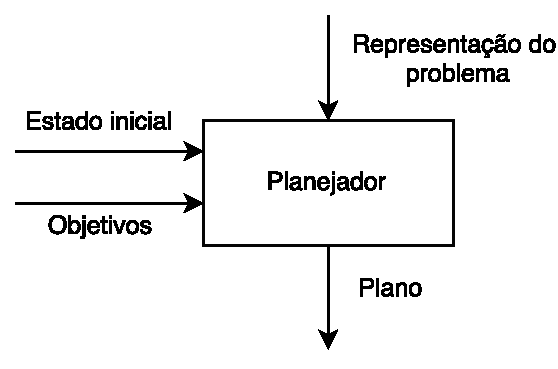
\includegraphics[width=0.4\textwidth]{fig/modelo.pdf}
	\caption{Problema de planejamento}
	\label{fig:planmodelo}
\end{figure} 

\section{HTN} 

Dentro da área de planejamento existe o planejamento hierárquico, chamado de \textit{Hierarchical Task Network} (HTN). HTN é igual ao planejamento clássico, quando se refere a representação do problema, entretanto o diferencial vem do que é planejado e como é planejado \cite{ghallab2004automated}, mas acaba sendo mais expressivo que o planejamento clássico, porque no planejamento clássico o conjunto de solução dos problemas é uma linguagem regular, ou seja, pode ser expressada por uma expressão regular, já em HTN dependendo da técnica utilizada o conjunto de solução dos problemas pode chegar a uma linguagem livre de contexto, que contém as linguagens regulares como um subconjunto, pois existem linguagens livres de contexto que não são linguagens regulares. No pior caso o resultado gerado do planejamento clássico será exponencialmente maior do que o gerado pelo planejamento HTN \cite{ghallab2004automated}.  

Em planejamento HTN as ações são tratadas em mais alto nível \cite{intelligence2003modern}. e o objetivo é achar um conjunto de tarefas que resolve determinado problema. Para isso, além da representação do problema, um conjunto de métodos é adicionado como entrada, onde este conjunto serve para decompor as tarefas em tarefas menores. O planejamento é feito decompondo tarefas não primitivas recursivamente até chegar em tarefas primitivas, que podem ser realizadas com um operador de planejamento \cite{ghallab2004automated}. Um método HTN é definido como \textit{m} = (nome(\textit{m}), tarefa(\textit{m}), subtarefas(\textit{m}), limitação(\textit{m})), onde cada elemento é definido como \cite{ghallab2004automated}: 

\begin{itemize}
	\item nome(\textit{m}) - Nome do método, que deve ser único, e \textit{m} é o conjunto de variaveis que será utilizado em \textit{m}. 
	\item tarefa(\textit{m}) - É uma tarefa não primitiva.
	\item (subtarefa(\textit{m}),limitação(\textit{m})) - É uma ligação de tarefa de ligação.
\end{itemize}

Uma tarefa de ligação é definida como um par w = (U,C), onde U é um conjunto de tarefas de ligação e C um conjunto de limitações. Cada limitação deve ser satisfeita em todo o plano e cada tarefa de ligação é decomposta em sub tarefas até todas as tarefas se tornarem primitivas. 

Um problema de planejamento HTN é descrito como P = ($s_{0}$, w, O, M), onde $s_{0}$ é o estado inicial, w a tarefa de ligação inicial, O é um conjunto de operadores de planejamento, e M é um conjunto de métodos. 

Na busca pelo plano, o planejamento HTN começa planejando por um caminho, quando um caminho de resolução leva a um fim de linha é realizado um retrocesso(\textit{backtracking}) até um caminho que tenha uma possibilidade diferente de caminho do que foi tomado anteriormente.


\section{AHTN} 

\textit{Adversarial hierarchical-task network} (AHTN) é um algoritmo proposto para tentar solucionar o problema do grande fator de ramificação dos jogos em tempo real \cite{ontanon2015adversarial}. Nele são combinados técnicas de HTN com o algoritmo \textit{minimax search}. O algoritmo \ref{alg:ahtn} é a representação da técnica de AHTN. Cada nodo da arvore das jogadas é definido por uma tupla $(s, N_{+}, N_{-}, t_{+}, t_{-})$, onde s é o estado corrente do ambiente, $N_{+}$ e $N_{-}$ são a representação de planos HTN para os jogadores max e min, respectivamente, $t_{+}$ e $t_{-}$ representam ponteiros para qual parte do plano HTN está sendo executado, sendo  $t_{+}$ uma tarefa de $N_{+}$ e $t_{-}$ uma tarefa de $N_{-}$. \textit{nextAction(N,t)} é uma função que, dado um HTN N e um ponteiro t, encontra a tarefa primitiva que deve ser executada em N. Se N ainda não estiver completamente decomposto, ou seja, ainda existem tarefas não primitivas, então \textit{nextAction(N,t)} = $\perp$.  $decompositions_{+}(s, N_{+}, N_{-}, t_{+}, t_{-})$ denota o conjunto das decomposições validas que adicionem apenas um novo método em $N_{+}$. A partir de uma função de avaliação, que pode ser aplicada sobre um estado, é retornado a recompensa de max em um estado terminal ou uma aproximação se o estado for não terminal. A partir destas definições, o algoritmo para AHTNMin é análogo. O algoritmo retorna o melhor plano encontrado para os dois jogadores, e também o resultado da função de avaliação no nodo terminal alcançado após a execução dos planos. A grande diferença entre o algoritmo de AHTN e o algoritmo do \textit{minimax search}, é que as chamadas recursivas nem sempre se alternam entre max e min. O algoritmo troca de nodos max para min apenas quando os planos estão totalmente decompostos a ponto de gerar uma ação. 

\begin{algorithm}
	\caption{AHTNMax(s, $N_{+}$, $N_{-}$, $t_{+}$, $t_{-}$, d)}
	\label{alg:ahtn}
	\begin{algorithmic}[1]
		\If {terminal(s) $\vee$ d $\leq$ 0}
		\State	\Return ($N_{+}$, $N_{-}$, e(s))
		\EndIf
		\If {nextAction($N_{+}$, $t_{+}$) $\neq$ $\perp$}
		\State t = nextAction($N_{+}$, $t_{+}$) 
		\State \Return AHTNMin($\gamma$(s,t), $N_{+}$, $N_{-}$, t, $t_{-}$, d-1)
		\EndIf
		\State $N_{+}^{*}$ = $\perp$, $N_{-}^{*}$ = $\perp$, $v^{*}$ = $-\infty$
		\State $\aleph$ = $decompositions_{+}(s, N_{+}, N_{-}, t_{+}, t_{-})$
		\ForAll{$N \in \aleph$}
		\State $(N^{'}_{+}, N^{'}_{-}, v^{'}) = AHTNMax(s, N, N_{-}, t_{+}, t_{-}, d)$
		\If{$v^{'} > v^{*}$}
		\State $N_{+}^{*} = N^{'}_{+}, N_{-}^{*} = N^{'}_{-}, v^{*} = v^{'} $
		\EndIf
		\EndFor		
		\State \Return $(N_{+}^{*}, N_{-}^{*}, v^{*} )$
	\end{algorithmic}
\end{algorithm}

